\clearpage
\section*{September 8, 2026: Construction payroll is higher in Manhattan}
\textit{Agent-drafted research entry.}

Private-sector construction establishments in Manhattan report substantially higher average weekly pay than those in the Bronx and Brooklyn. In 2023, the respective amounts were \$2,377, \$1,712, and \$1,385. The same ordering appears in 2019, before the pandemic: \$2,088, \$1,467, and \$1,212. These are nominal dollars within each year.

The difference persists within residential building construction. In 2023, Manhattan reported \$1,983 per week, compared with \$1,197 in the Bronx and \$1,239 in Brooklyn. Heavy and civil engineering is an exception: Bronx pay exceeds Manhattan pay in 2023. Industry composition therefore matters, but it does not account for the entire Manhattan difference.

The Quarterly Census of Employment and Wages provides all 125 requested cells: five boroughs, five years from 2019 through 2023, and five overlapping construction categories. No selected cell is suppressed or absent. The audit preserves published annual employment, payroll, and pay measures and checks the payroll identity allowing for rounding. The standard data report establishes the first baseline for this source.

These findings are consistent with the proposed wage mechanism but do not establish it. Payroll includes all occupations within an industry, and average weekly pay reflects hours and workforce composition. Establishment addresses can locate the contractor's office rather than the construction site. These data do not directly measure the hourly compensation paid on a particular development. Jacob requested this public-data check in audits; a custom NY Department of Labor request remains deferred.

\textit{Reproduction:} Run Make in the code directory of
\texttt{tasks/audits/audit\_qcew\_construction\_wages}.
The acquisition task retains BLS annual county CSV slices retrieved September 8, 2026, with source fingerprints in its reports. Private ownership and all establishment sizes are selected. NAICS categories are 23, 236, 2361, 237, and 238; they must not be summed. Code is an uncommitted audit addition to revision 7bbf6d5.

\clearpage
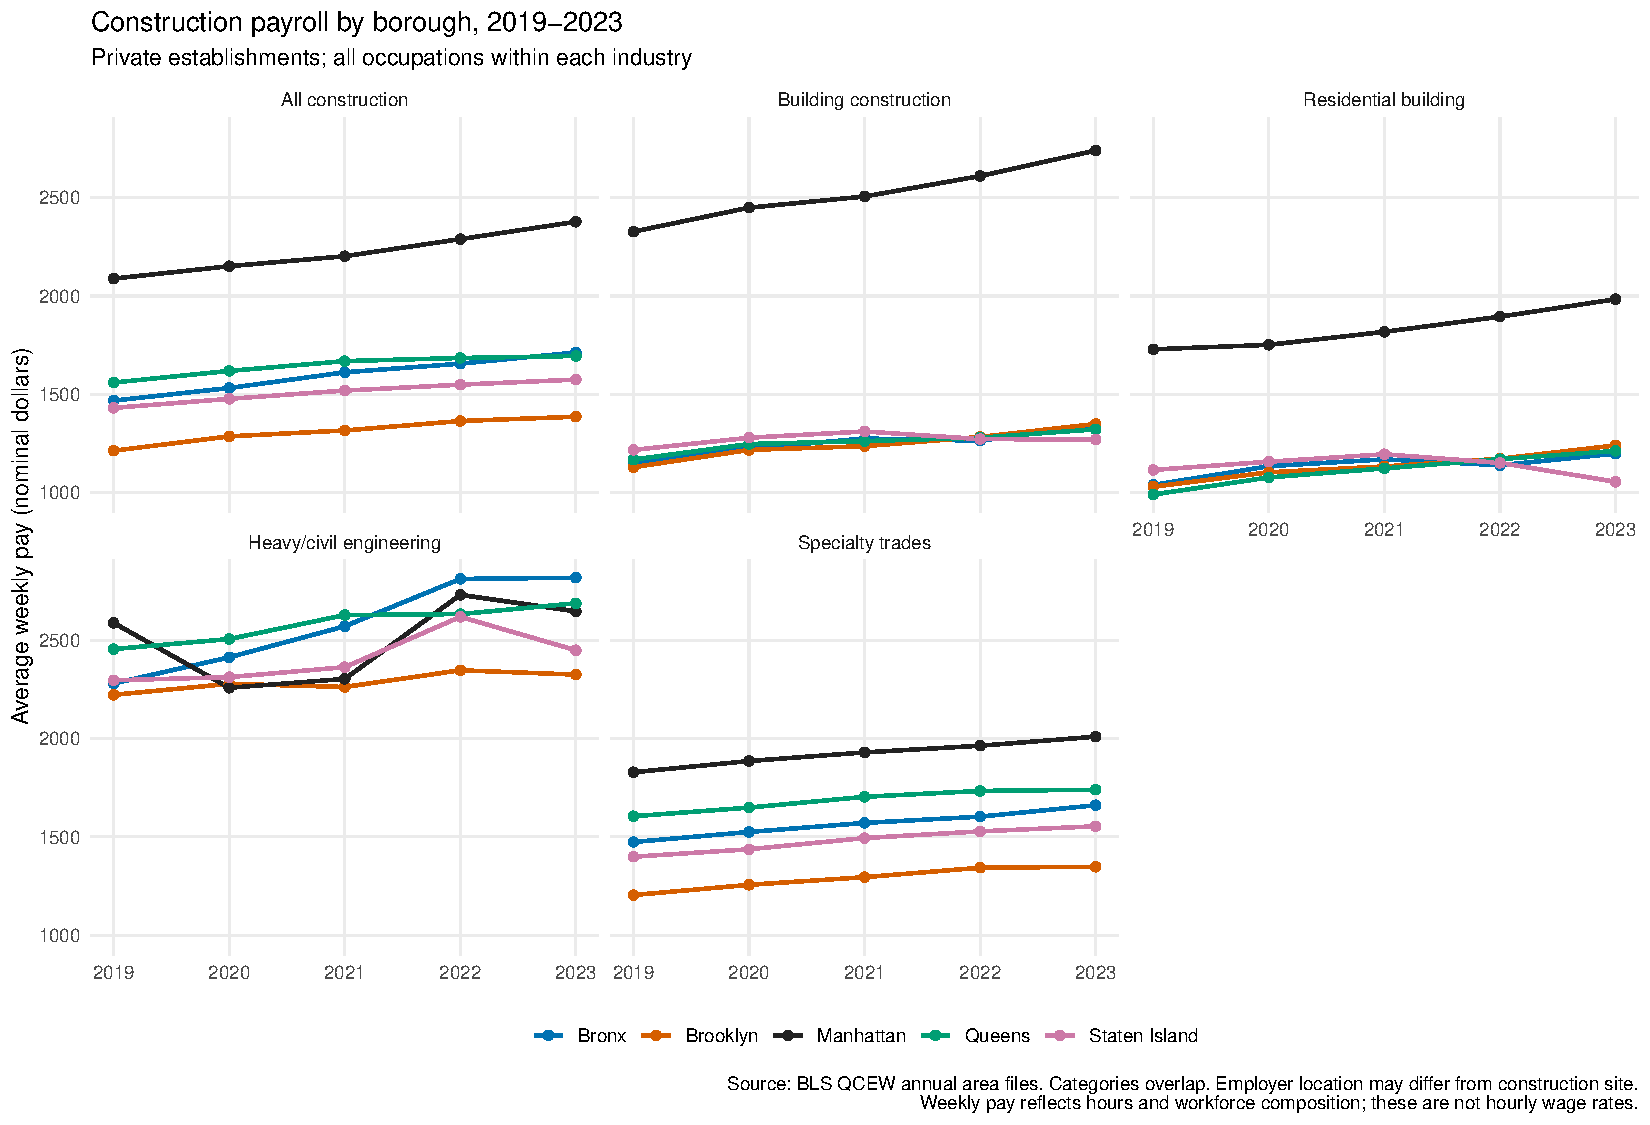
\includegraphics[width=\textwidth,page=1]{archive/2026-09-08-wage-feasibility/borough_construction_pay.pdf}
\clearpage
\includegraphics[width=\textwidth,page=2]{archive/2026-09-08-wage-feasibility/borough_construction_pay.pdf}
